\documentclass[aspectratio=169,14pt]{beamer}
\usepackage{zxjatype}
\usepackage[ipa]{zxjafont}
\title{BIND 9.11's new features\\
(BIND 9.11 新機能)}
\author{Mukund Sivaraman\\
~\\
\small muks@isc.org}
\institute{Internet Systems Consortium}
\date{}
\usenavigationsymbolstemplate{}

\begin{document}

\frame{\titlepage}

\frame
{
  \frametitle{New in BIND 9.11}

  \begin{itemize}

  \item Provisioning
    \begin{itemize}
    \item Catalog Zones
    \item DynDB
    \item \texttt{rndc showzone}, \texttt{modzone} and NZD backend
    \end{itemize}

  \item DNSSEC
    \begin{itemize}
      \item Negative trust anchors
      \item Child CDS/CDNSKEY automatic generation
      \item DNSSEC key manager
    \end{itemize}

  \item Other
    \begin{itemize}
    \item dnstap logging
    \item EDNS CLIENT-SUBNET (authoritative)
    \item Performance improvements
    \end{itemize}
  \end{itemize}
}

\frame
{
  \frametitle{Provisioning}

  \begin{itemize}

  \item Before Catalog Zones, operators didn't have any way to
    automatically create a new zone on a slave server to match a new
    zone on a master, other than accessing the slave's configuration
    file and executing a reconfig.

  \item Operators wanted \textbf{standardized provisioning} that didn't
    require maintaining custom scripts and methods for updating slaves.

  \item Some operators wanted ability to serve zone data from a shared
    database backend.

  \item BIND administrators found that deleting zones when using
    \textbf{NZF config files} (\textbf{rndc delzone}) was slow when the
    number of zones was large.

  \end{itemize}
}

\frame
{
  \frametitle{Catalog Zones}

  \begin{itemize}

  \item A \textbf{DNS catalog} is a list of zones.

  \item A \textbf{catalog zone} is a regular DNS zone that contains the
    list of zones represented as regular RRs within the zone.

  \item Slaves transfer this zone from the master and
    \textbf{reconfigure automatically} to serve the list of zones within
    the catalog.

  \item When a zone name is added to the catalog zone on the master, the
    catalog zone update is transferred to the slaves. The slave then
    adds the new zone to its configuration automatically and transfers
    the new zone's contents from the master.

  \item We are trying to standardize the method as
    \texttt{draft-muks-dnsop-dns-catalog-zones-01}.

  \end{itemize}
}

\frame
{
  \frametitle{Catalog Zone Example}

\texttt{cat.isc.org. IN SOA . . 2016022901 900 600 86400 1}\\
\texttt{cat.isc.org. IN NS nsexample.}\\
~\\
\texttt{version.cat.isc.org. IN TXT "1"}\\
~\\
\texttt{5960775b5c.zones.cat.isc.org. IN PTR domain1.com.}\\
\texttt{0e2ffd0d66.zones.cat.isc.org. IN PTR domain2.net.}\\
\texttt{ab89bcd650.zones.cat.isc.org. IN PTR domain3.org.}

}

\frame
{
  \frametitle{DynDB - dynamic DB interface}

  \begin{itemize}

  \item \textbf{dns\_db} C API interface is used by \textbf{named} to
    store zone data, and access zone data when serving DNS queries.

  \item \textbf{RBTDB} is the default statically linked \textbf{dns\_db}
    implementation within \textbf{named} that is used to store zone
    contents in memory.

  \item \textbf{DynDB} allows administrators to install other
    \textbf{dns\_db} implementations as dynamically loadable
    \textbf{.so} modules that provide other backends such as SQL
    databases, customized answer generation, etc. Such modules are
    called \textbf{drivers}.

  \item Currently there are no drivers in BIND 9.11. We hope that some
    will be contributed for open source SQL databases.

  \end{itemize}
}

\frame
{
  \frametitle{Negative Trust Anchors}

  \begin{itemize}

    \item \textbf{rndc nta} command can be used to \textbf{temporarily}
      disable DNSSEC validation for a domain for a specific duration.

    \item This is useful to a resolver operator in case a popular domain
      is failing DNSSEC validation temporarily and gets complaints from
      users that they are not able to resolve names within that zone.

    \item \textbf{named} will periodically test to see whether data
      below an NTA can now be validated.

    \item The negative trust anchor expires after the configured time.

  \end{itemize}
}

\frame
{
  \frametitle{Child CDS/CDNSKEY automatic generation}

  \begin{itemize}

  \item BIND now automatically creates CDS and CDNSKEY records, signed
    by the KSK.

  \item The parent side of a delegation can poll the child zone for
    these CDS and CDNSKEY and automatically update DS records on the
    parent.

  \item This allows rolling the KSK without requiring a manual update of
    the DS record in the parent zone.

  \item Note that BIND does not currently implement parent-side behavior
    of automatically updating the DS records.

  \end{itemize}
}

\frame
{
  \frametitle{\texttt{dnssec-keymgr} - DNSSEC key manager}

  \begin{itemize}

  \item Python wrapper tool to facilitate the key rollover process for
    zones handled by BIND. It calls BIND utilities.

  \item Reads a policy definition file (default:
    \texttt{/etc/dnssec.policy}) and creates or updates DNSSEC keys to
    ensure that a zone's keys match the policy for that zone.

  \item New keys are created when necessary.

  \item Existing keys' timing metadata is adjusted as needed to set the
    correct rollover, etc.

  \item If the policy changes, all applicable keys are corrected.

  \item It is expected that this tool will be run automatically and
    unattended (for example, using \texttt{cron}).

  \end{itemize}
}

\frame
{
  \frametitle{EDNS CLIENT-SUBNET}

  \begin{itemize}

  \item A basic experimental implementation of authoritative
    CLIENT-SUBNET has been added in 9.11.

  \item During 9.11 development cycle, we also implemented resolver EDNS
    CLIENT-SUBNET support for BIND which is complete and ready for
    production use, but we cannot release it currently due to
    contractual reasons. We plan to make it available to subscription
    users, but it will not be released in public releases until some
    time in 2018.

  \end{itemize}
}

\frame
{
  \frametitle{Changes to BIND development process}

  \begin{itemize}

  \item Performance lab.

  \item Fuzz testing.

  \end{itemize}
}

\frame
{
  \frametitle{Perflab - continuous benchmarking}

  \begin{center}
    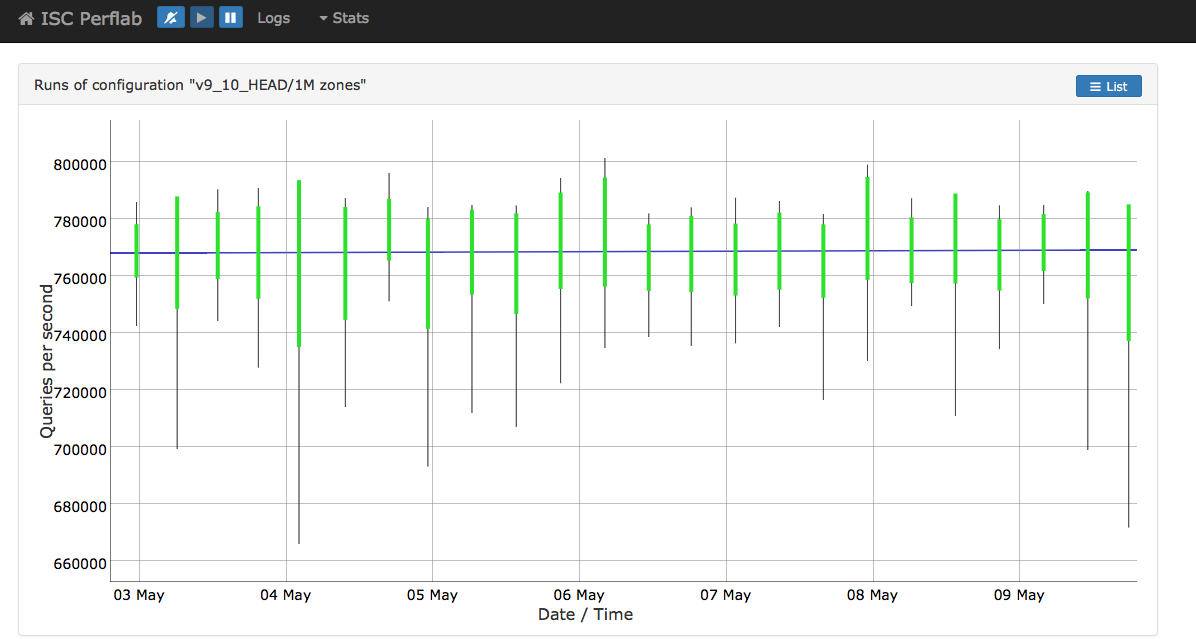
\includegraphics[scale=0.3]{perf1.png}
  \end{center}
}

\frame
{
  \frametitle{Perflab - list of tests}

  \begin{center}
    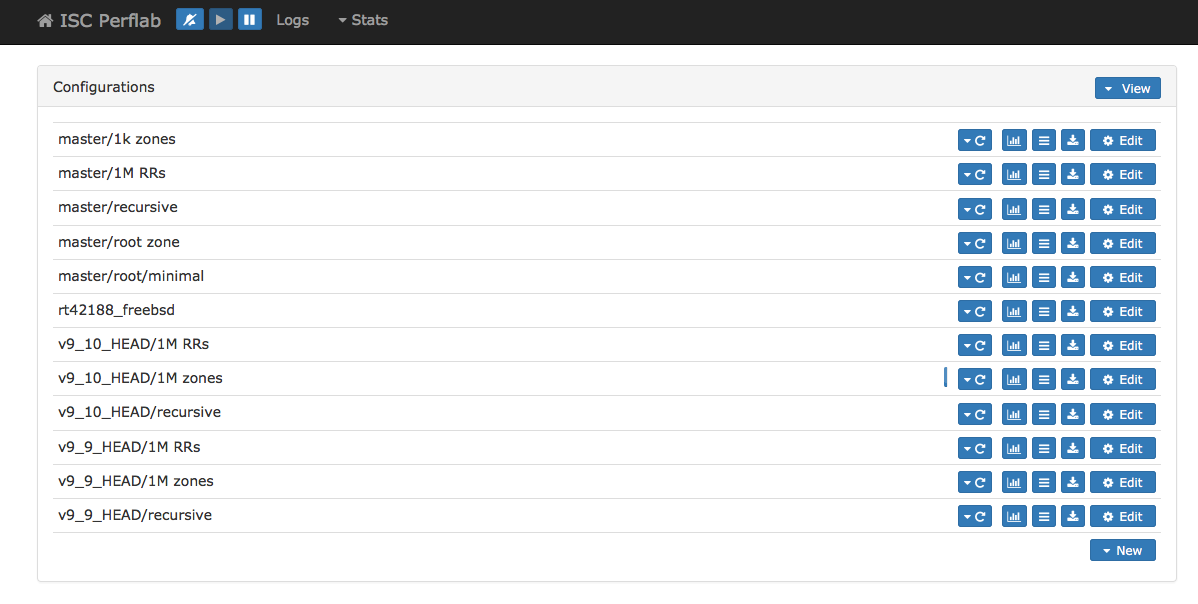
\includegraphics[scale=0.3]{perf2.png}
  \end{center}
}

\frame
{
  \frametitle{Perflab - noticing QPS changes}

  \begin{center}
    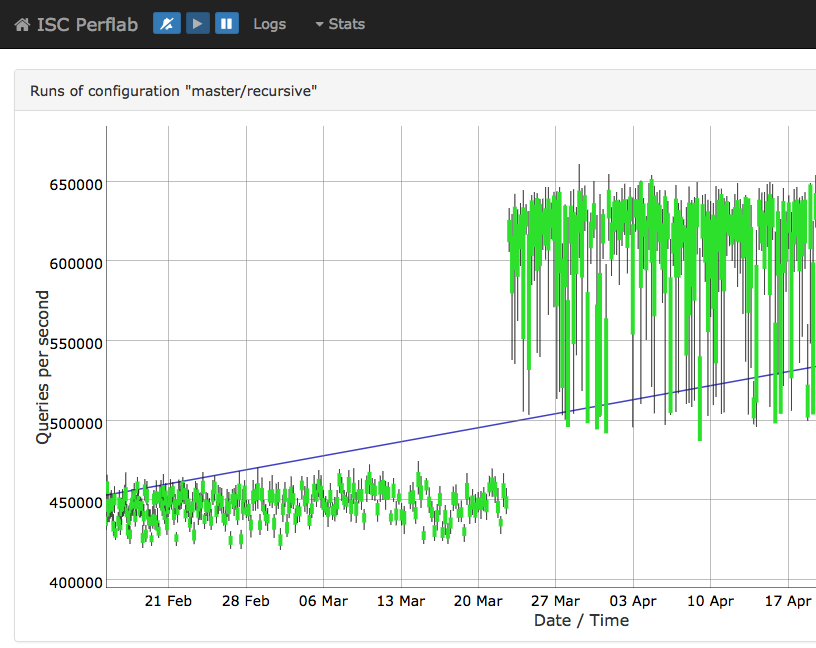
\includegraphics[scale=0.3]{perf3.png}
  \end{center}
}

\frame
{
  \frametitle{Fuzzing and CVE announcements}

  \begin{itemize}

  \item ISC has been fuzz testing BIND to find defects pro-actively.

  \item Over the past year, CVEs have been issued for bugs found
    internally by fuzzing and code review.

  \item Patch is always available for users with a CVE
    announcement. JPRS makes Japanese translations of release
    announcements: \url{https://jprs.jp/tech/}

  \item OS distributions are given notice to prepare patched packages in
    advance so users can upgrade on announcement day.

  \item Most of these CVE bugs (crash-capable) were introduced many
    years ago. Quality of the codebase is increasing as we remove these
    bugs and refactor code.

  \end{itemize}

}

\frame
{
  \frametitle{End}

  \begin{itemize}

  \item We want feedback from Japanese community. We see many issues
    discussed on Twitter in Japanese language.

  \item Discuss issues on bind-users mailing list:
    \url{https://lists.isc.org/mailman/listinfo/bind-users}

  \end{itemize}

}

\end{document}
